\documentclass[11pt]{article}

\usepackage[margin=1in]{geometry}
\usepackage[T1]{fontenc}
\usepackage{lmodern}
\usepackage{microtype}
\usepackage{amsmath,amssymb}
\usepackage{booktabs}
\usepackage{graphicx}
\usepackage{xcolor}
\usepackage[numbers,sort&compress]{natbib}
\usepackage{tikz}
\usetikzlibrary{positioning,arrows.meta,fit,calc}
\usepackage[colorlinks=true,linkcolor=blue!60!black,citecolor=blue!60!black,urlcolor=blue!60!black]{hyperref}
\usepackage{cleveref}

\newcommand{\M}{\texttt{[M]}}

\title{\textbf{HALE-LLM: Autoregressive, Masked Diffusion, Block Diffusion and\\Discrete Flow Matching on One Transformer Backbone}}
\author{B A NaveenKumar\\
\small Independent researcher\\
\small \url{https://github.com/basaanithanaveenkumar/Hale-LLM}}
\date{}

\begin{document}
\maketitle

\begin{abstract}
Masked diffusion and related non-autoregressive language models have become credible
alternatives to next-token prediction, but published comparisons usually differ in more
than the objective: backbone, tokenizer, data pipeline and evaluation all change at once.
\textbf{HALE-LLM} is a controlled testbed in which the \emph{paradigm} is a plugin and
everything else is shared. It includes autoregressive (AR) next-token prediction,
absorbing-state masked diffusion, block diffusion (autoregressive across blocks, diffusion
within a block) and a masking-path discrete flow matching variant, with a multi-token
prediction stub. Every paradigm uses the same modular decoder library (MHA/GQA/MQA, RoPE,
dense, GeGLU or mixture-of-experts FFN, and GPT, local--global or DiT stacks), the same
GPT-2 tokenizer and WikiText-2 pipeline, the same metrics (loss, perplexity or ELBO bound,
bits per token, token and masked accuracy) and the same experiment tooling with
per-step unmasking visualisations. Masking is a configuration switch (causal,
bidirectional or block-causal), as are the attention implementation and the backbone. We
describe the objectives exactly as implemented, show that the flow-matching variant
coincides with masked diffusion under a time reparameterisation, report measured model
sizes and give a qualitative block-diffusion decoding trace.
\end{abstract}

\section{Introduction}

Autoregressive transformers~\cite{vaswani2017attention,radford2019gpt2} generate one token at a
time, left to right. Discrete diffusion models~\cite{austin2021d3pm,lou2024sedd} instead corrupt
text and learn to reverse the corruption. The \emph{absorbing-state} (masking) variant has
emerged as the simplest and strongest~\cite{sahoo2024mdlm,shi2024md4}, and it now scales to
billions of parameters~\cite{nie2025llada}. Block diffusion~\cite{arriola2025bd3lm}
interpolates between the two, and discrete flow matching~\cite{gat2024dfm} offers another view of
the same family. Multi-token prediction~\cite{gloeckle2024mtp} keeps left-to-right order but
predicts several tokens per step.

Comparisons between these paradigms are hard to read when the backbone and data also change.
HALE-LLM fixes everything except the paradigm. Our contributions:
\begin{itemize}
  \item A \textbf{paradigm-as-plugin architecture}: each paradigm is a folder with a model, a
        collate function, a loss, a sampler and optional metrics, registered by name. Shared
        code never imports a paradigm (\cref{sec:system}).
  \item \textbf{Exact objectives} for AR, masked diffusion, block diffusion and flow matching
        as implemented, including the ELBO weights and the block-causal attention mask
        (\cref{sec:objectives}).
  \item A \textbf{shared modular backbone} in which masks, attention type, FFN and stack
        (GPT, Gemma-3-style local--global, DiT) are switches (\cref{sec:backbone}).
\end{itemize}

\section{Paradigms}
\label{sec:objectives}

Let $x=(x^1,\dots,x^L)$ be a token sequence, \M\ a special mask token, and
$f_\theta$ the backbone producing per-position logits. All losses use the same per-token
negative log-likelihood (cross-entropy by default, focal optional) and ignore padding.

\paragraph{Autoregressive.} Causal mask, and the collate shifts labels so that position $\ell$
predicts $x^{\ell+1}$: $\mathcal L_{\text{AR}} = -\frac1L\sum_\ell \log p_\theta(x^{\ell+1}\mid x^{\le \ell})$.

\paragraph{Masked diffusion.} With the log-linear schedule $\alpha_t=1-t$, each token is
independently replaced by \M\ with probability $t\sim\mathcal U(\epsilon,1)$. A bidirectional,
time-conditioned backbone predicts the clean tokens, and the MDLM continuous-time
ELBO~\cite{sahoo2024mdlm,shi2024md4} weights masked-position cross-entropy by
$-\alpha'_t/(1-\alpha_t)=1/t$:
\begin{equation}
  \mathcal L_{\text{MD}} = \mathbb E_{t,x_t}\Big[\tfrac1t \textstyle\sum_{\ell: x_t^\ell=\M} -\log p_\theta(x^\ell\mid x_t, t)\Big],
\end{equation}
normalised by the number of masked, non-pad positions. Sampling starts from an all-mask
continuation after the prompt and walks a grid $1=t_0>\dots>t_S=\epsilon$. At each step
every masked position is revealed with probability $(t_i-t_{i+1})/t_i$, using a token sampled
from the temperature-scaled prediction with \M\ excluded.

\paragraph{Block diffusion.} The sequence is split into blocks of $B$ tokens (16 by default).
Each block $k$ gets its own noise level $t_k$ and is masked independently. The model receives
the clean sequence and the noised sequence concatenated ($2L$ tokens, clean time $=0$) under a
block-causal mask~\cite{arriola2025bd3lm}. Clean tokens attend to clean tokens in their own
and earlier blocks, and noisy tokens attend to clean tokens in \emph{strictly earlier} blocks
and to noisy tokens in their own block. The loss is the MD loss over noisy positions with
weight $1/t_k$. Generation is autoregressive over blocks: for each block not covered by the
prompt, $S$ reveal steps run with $t$ going from 1 to 0 inside the block while earlier
blocks stay fixed.

\paragraph{Discrete flow matching (masking path).} Time runs the other way: $t=0$ is the fully
masked source and $t=1$ the data. Tokens are masked with probability $1-t$,
$t\sim\mathcal U(0,1-\epsilon)$, and masked-position cross-entropy is weighted by
$1/(1-t)$. Substituting $s=1-t$ recovers exactly the masked-diffusion corruption and
weight, so under this linear masking path the two objectives are the same up to time
reparameterisation and the range of $t$~\cite{gat2024dfm,shi2024md4}. Keeping both as separate
plugins is still useful. The flow parameterisation is where non-linear or
non-absorbing paths (a documented extension point) diverge from MDLM.

\paragraph{Multi-token prediction (stub).} The MTP variant allocates $n-1$ extra heads but
currently trains only the main next-token head. The multi-head loss and a self-speculative
decoder~\cite{gloeckle2024mtp} are future work.

\section{Shared Backbone}
\label{sec:backbone}

The decoder library (\texttt{ha\_llm.core}) provides attention (MHA, GQA~\cite{ainslie2023gqa},
MQA~\cite{shazeer2019mqa}, RoPE~\cite{su2021roformer}, optional QK-norm), FFNs (GELU MLP,
GeGLU~\cite{shazeer2020glu}, DeepSeek-style MoE~\cite{dai2024deepseekmoe}), RMSNorm~\cite{zhang2019rmsnorm},
and three stacks. The \textbf{GPT} stack is pre-LayerNorm with learned positions. The
\textbf{LGT} stack follows Gemma~3~\cite{gemma3}: five sliding-window local layers with RoPE
$\theta=10^4$ per global layer with $\theta=10^6$ and partial RoPE. The \textbf{DiT} stack uses
AdaLN-Zero~\cite{peebles2023dit}. Time conditioning (a sinusoidal embedding followed by an MLP)
modulates every layer's norms for the diffusion-family paradigms. The LM head is tied to the
token embedding.

\Cref{tab:configs} lists the shipped configurations. All share $d=384$, 16 layers, 8 heads,
$d_{ff}=1536$, 128 tokens, dropout 0.1 and the GPT-2 tokenizer extended with \M\
($V=50{,}258$).

\begin{table}[t]
\centering
\caption{Shipped configurations (parameter counts measured from the code).}
\label{tab:configs}
\small
\begin{tabular}{llllr}
\toprule
Paradigm & Stack & Attention & Mask & Params \\
\midrule
Autoregressive & GPT, MLP & MHA & causal & 47.7M \\
Masked diffusion & LGT, GeGLU, time-cond. & GQA ($n_{kv}{=}2$) & bidirectional & 63.2M \\
Block diffusion ($B{=}16$) & LGT, GeGLU, time-cond. & GQA & block-causal & 63.2M \\
Flow matching & LGT, GeGLU, time-cond. & GQA & bidirectional & 63.2M \\
\bottomrule
\end{tabular}
\end{table}

\section{System}
\label{sec:system}

\begin{figure}[t]
\centering
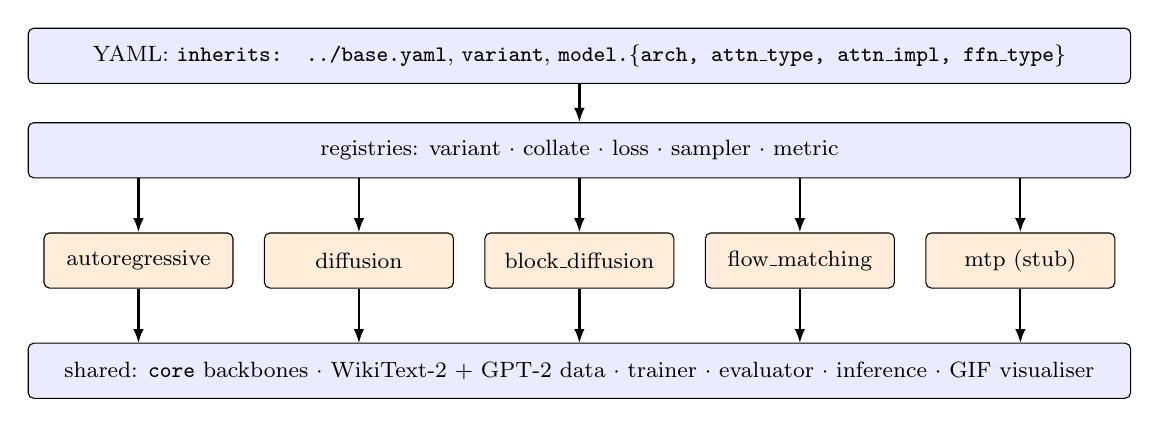
\begin{tikzpicture}[
  box/.style={draw, rounded corners=2pt, align=center, font=\footnotesize, minimum height=7mm, inner sep=3pt},
  sh/.style={box, fill=blue!8, minimum width=140mm},
  pl/.style={box, fill=orange!15, minimum width=24mm},
  arr/.style={-{Latex[length=1.8mm]}, thick}
]
\node[sh] (yaml) at (0,0) {YAML: \texttt{inherits: ../base.yaml}, \texttt{variant}, \texttt{model.\{arch, attn\_type, attn\_impl, ffn\_type\}}};
\node[sh] (reg) at (0,-1.2) {registries: variant $\cdot$ collate $\cdot$ loss $\cdot$ sampler $\cdot$ metric};
\foreach \n/\x/\lab in {ar/-5.6/autoregressive, md/-2.8/diffusion, bd/0/block\_diffusion, fm/2.8/flow\_matching, mtp/5.6/mtp (stub)} {
  \node[pl] (\n) at (\x,-2.6) {\lab};
  \draw[arr] (\x,-1.55) -- (\n.north);
  \draw[arr] (\n.south) -- (\x,-3.65);
}
\node[sh] (core) at (0,-4.0) {shared: \texttt{core} backbones $\cdot$ WikiText-2 + GPT-2 data $\cdot$ trainer $\cdot$ evaluator $\cdot$ inference $\cdot$ GIF visualiser};
\draw[arr] (yaml) -- (reg);
\end{tikzpicture}
\caption{Paradigms are plugins registered by name. Shared code never imports them directly.}
\label{fig:system}
\end{figure}

\Cref{fig:system} shows the structure. A run is a strict YAML configuration (unknown keys are
rejected) that inherits \texttt{base.yaml}. The \texttt{variant} key selects the registered model,
collate, loss, sampler and variant-specific metrics. Data come from Hugging Face
(WikiText-2 raw~\cite{merity2017wikitext} by default), tokenised with GPT-2 and cut into
128-token windows with a 10-word sliding stride. Each run gets a timestamped directory
containing the resolved and source configurations, checkpoints, logs, TensorBoard events and
visualisation GIFs, and a \texttt{latest} symlink enables resuming. Four CLIs cover training,
sampling, evaluation and visualisation. Evaluation reports loss, perplexity (an upper bound
via the ELBO for diffusion-family models), bits per token, token accuracy, top-$k$ accuracy
and masked accuracy.

\section{Qualitative Decoding Trace}

\begin{figure}[t]
\centering
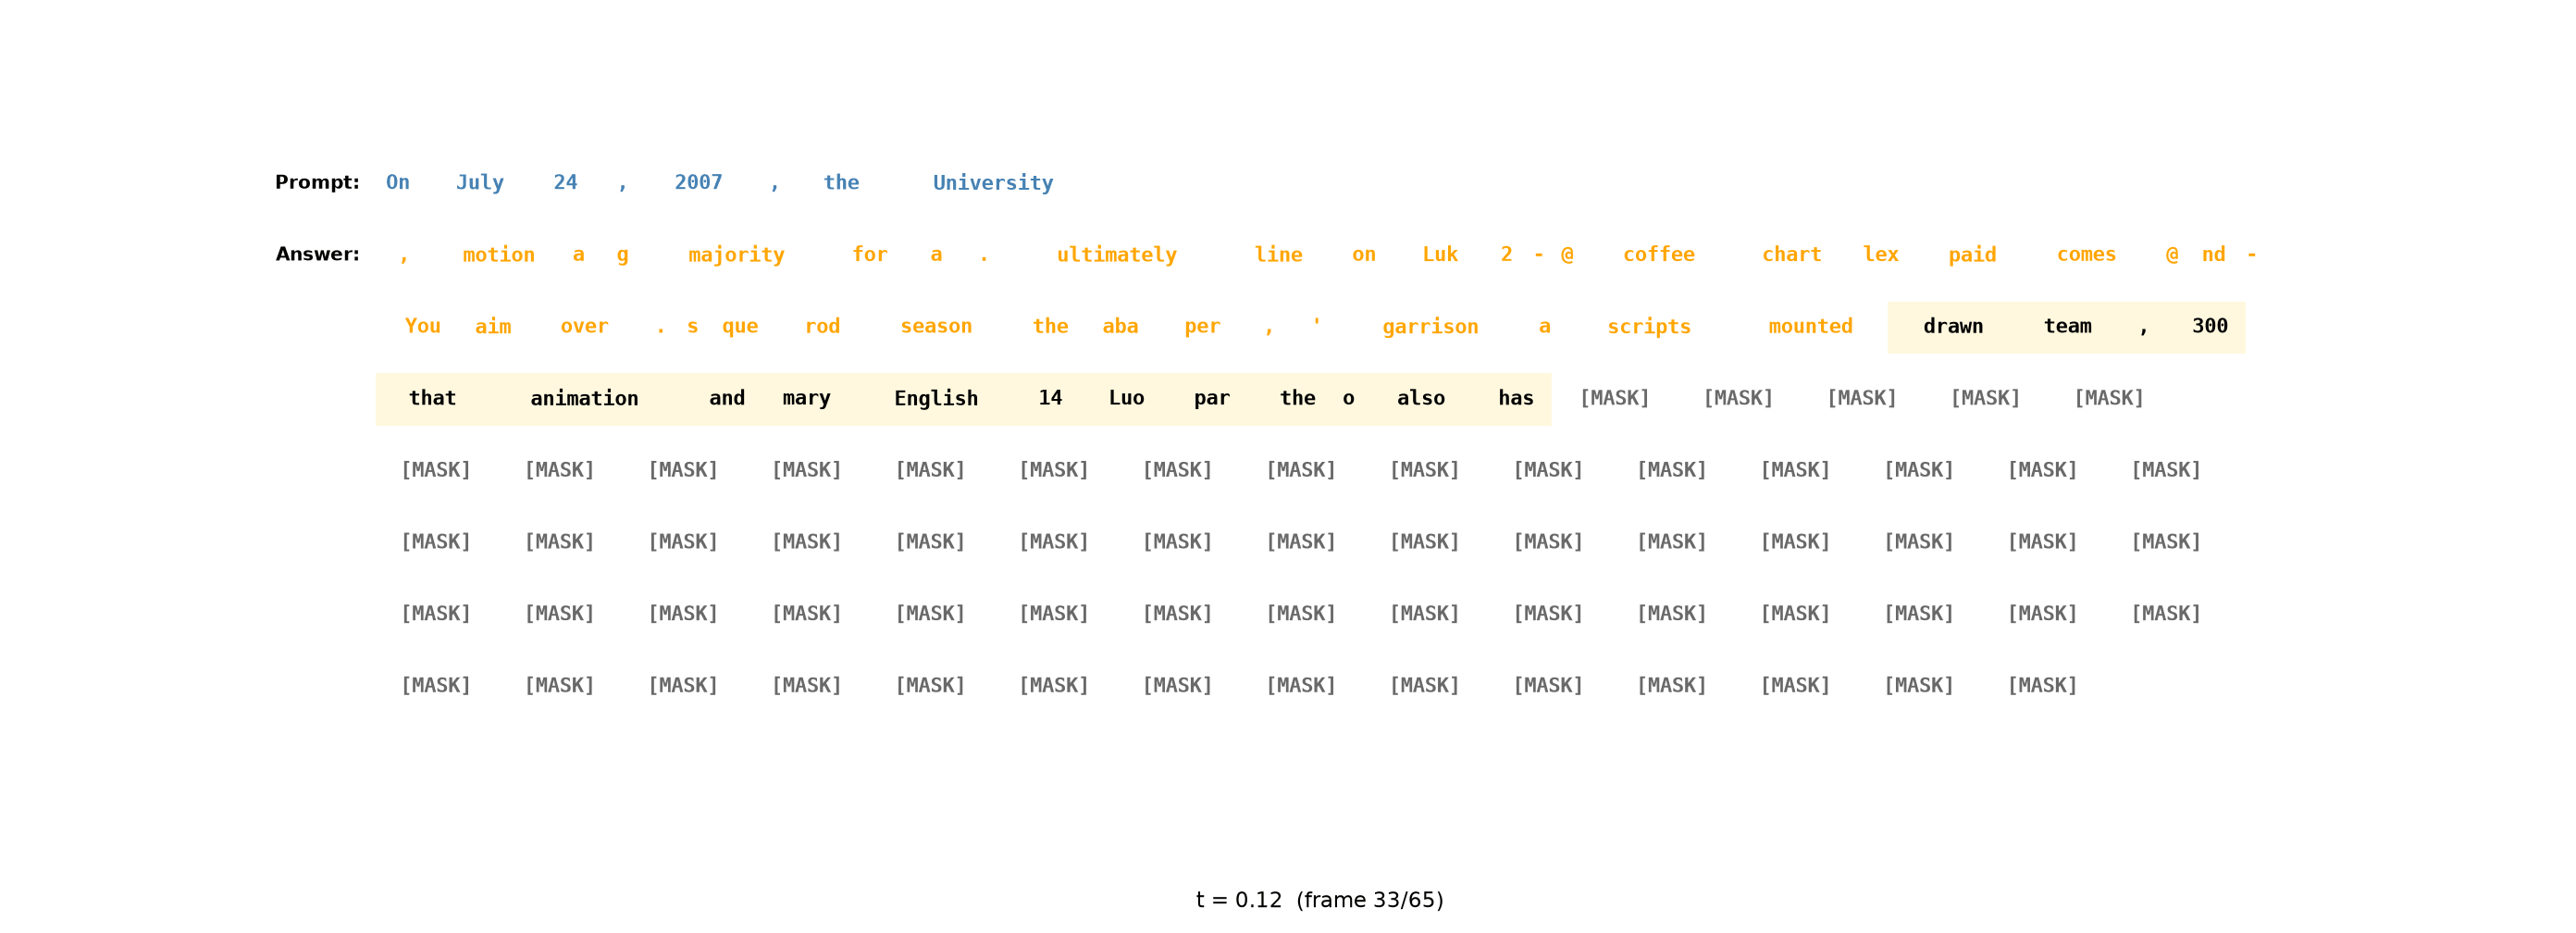
\includegraphics[width=\linewidth]{figures/block_diffusion_mid.png}
\caption{Block diffusion decoding on a WikiText-2 prompt at training step 4{,}900 (frame 33 of
65 from the repository's visualiser). Blue: prompt. Orange: committed tokens from earlier
blocks. Highlighted: the block being denoised. Grey: still masked. Tokens are committed block
by block, left to right. At this early checkpoint the output has WikiText-like vocabulary
and punctuation (including the corpus's \texttt{@-@} artefacts) but is not yet coherent.}
\label{fig:bd}
\end{figure}

\Cref{fig:bd} shows the block-wise generation order produced by the block-causal mask and
sampler: previous blocks are frozen while the current block is progressively unmasked. The
sample comes from an early checkpoint of a small model and is shown to illustrate the
decoding process, not quality.

\section{Status and Limitations}

% TODO: add quantitative comparisons only when produced by ha-llm-eval runs in this repo.
We do not yet report quantitative comparisons. The intended protocol is equal-size models
trained for equal steps on WikiText-2, comparing validation bits per token (exact for AR, an
ELBO bound for the diffusion family), sample quality against the number of sampling steps,
and the effect of block size. Current limitations: the MTP variant is a stub; the
flow-matching variant uses only the masking path, which makes it equivalent to masked
diffusion; the samplers use simple random reveal orders with no confidence-based remasking;
and three unit tests still reference the repository's former package name and fail at
import. The remaining 53 unit tests pass.

\section{Conclusion}

HALE-LLM reduces the difference between language-modelling paradigms to the part that
actually differs, which is the corruption process, the loss weighting and the sampler, and
shares the rest. We hope it makes comparisons between AR, diffusion, block diffusion and
flow matching at small scale easier to trust.

\bibliographystyle{plainnat}
\bibliography{references}

\end{document}
